V resničnem svetu pinhole kamere niso praktične, ker je slika zamegljena, če je odprtina prevelika, in pretemna, če je premajhna. Zato uporabljamo leče, ki vhodne žarke preusmerijo na slikovno ravnino. Zaradi uporabe leč pride do popačenja. Tukaj bomo obravnavali radialno in tangencialno popačenje. \\
Naj bodo $(x, y)$ koordinate točke na nepopačeni sliki in $(x_d, y_d)$ koordinate te iste točke na popačeni sliki. \\
Radialno popačenje povzroča ``barrel" ali ``fish-eye" efekt v slikah. Radialno popačenje lahko predstavimo kot
\begin{gather}
    x_d = x(1 + k_1 r^2 + k_2 r^4 + k_3 r^6) \notag\\
    y_d = y(1 + k_1 r^2 + k_2 r^4 + k_3 r^6) \notag\\
    r^2 = x^2+y^2
    \label{radialdistEq}
\end{gather}
\begin{figure}[h]
    \centering
    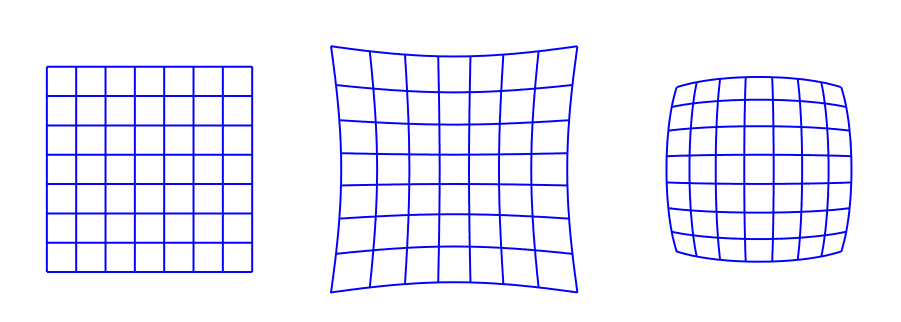
\includegraphics[width=0.5\linewidth]{imgs/radialdist.png}
    \caption{Radialno popačenje\cite{Tomasi_2025a}}
    \label{fig:raddist}
\end{figure}

Tangencialno popačenje nastane, ker leče niso popolnoma vzporedne s slikovno ravnino, in ga lahko predstavimo kot
\begin{gather}
    x_d = x+[2p_1xy+p_2(r^2+2x^2)] \notag\\
    y_d = y+[p_1(r^2+2y^2)+2p_2xy]
    \label{tangentialdistEq}
\end{gather}

Da bi ugotovili koeficiente popačenja $(k_1, k_2, p_1, p_2, p_3)$ ter notranje in zunanje parametre, izvedemo kalibracijo kamere\cite{calibtut}.